\documentclass[oneside]{book}

\usepackage[utf8]{inputenc}
\usepackage{graphicx}
\usepackage[russian]{babel}
\usepackage{indentfirst}
\usepackage{misccorr}
\usepackage[left=2cm,right=2cm,
    top=2cm,bottom=2cm,bindingoffset=0cm]{geometry}

\usepackage{amsmath}
\usepackage{mathrsfs}
\usepackage{enumitem}
\setlist[enumerate,1]{label=\arabic*.}

% Колонтитулы с названием главы и нумерация
\usepackage{fancyhdr}
\pagestyle{fancy}

% Если хочется, чтобы в оглавлении были только главы, и ничего ниже
\setcounter{secnumdepth}{-1} 

% Если есть картинки
\usepackage{graphicx}
\DeclareGraphicsExtensions{.jpg,.png,.gif}

% Если хочется гиперссылок в книге 
% (в макете для печатного издания они бессмысленны, конечно).
\usepackage{hyperref}


\begin{document}

\title{Дебильники по ДА}

\maketitle

\chapter{2015 год}

\section{Вариант 1 (июнь 2015)}
\begin{enumerate}
\item Приведите пример семейства 5-элементных множеств, имеющего ровно 2 минимальных системы общих представителей.
\item Во скольких связных графах на $20$ пронумерованных вершинах с 19 ребрами нет ни одного цикла?
\item Сформулируйте критерий наличия в графе эйлерового пути.
\item Найдите сумму всех элементов матрицы Адамара размера $8 \times 8$, первая строка которой состоит из единиц.
\item Нарисуйте связный граф без петель и кратных ребер, в котором нет гамильтонова пути.
\item Найдите хроматическое число любого графа на 7 вершинах с 20 ребрами.
\item Найдите $VC(\mathbb{Q}, F)$, где $F$ -- семейство всех бесконечных подмножеств множества $\mathbb{Q}$.
\item Приведите пример такой функции $f(n)$, что при $n \rightarrow \infty$ одновременно $f(n) = o(2^n)$ и $n^{2 \ln n} = o(f(n))$.
\end{enumerate}

\section{Вариант 2 (июнь 2015)}
\begin{enumerate}
\item Вычислите $R(3, 3, 2)$.
\item Найдите максимально возможное число ребер в графе с $15$ вершинами и кликовым числом $2$.
\item Напишите формулировку теоремы Эрдеша-Ко-Радо.
\item Найдите перманент матрицы $10 \times 10$, в которой 99 единиц и один ноль.
\item Сколько ребёр может быть у связного графа без петель и кратных рёбер с $50$ вершинами, если он нарисован на плоскости, причем его рёбра пересекаются только в вершинах и он делит плоскость на $11$ частей?
\item Нарисуйте дерево, кодом Прюфера которого является последовательность $(7, 6, 7, 6, 1, 1, 1)$.
\item Найдите $VC(\mathbb{N}, F)$, где $F$ -- семейство всех трёхэлементных подмножеств множества $\mathbb{N}$.
\item Найдите предел при $n \rightarrow \infty$ величины $\sqrt[n]{C_n^{n/4}}$.
\end{enumerate}

\section{Вариант 3 (июнь 2015)}
\begin{enumerate}
\item Какое неравенство связывает хроматическое число $\chi(G)$ и кликовое число $\omega (G)$ графа $G$?
\item Сформулировать достаточное условие Дирака гамильтоновости графа.
\item Нарисуйте связный граф без петель и кратных рёбер, в котором нет ни эйлерова пути, ни эйлерова цикла. 
\item Найти перманент матрицы, состоящей из $3$ столбцов и $6$ строк, у которой первый столбец состоит из единиц, а остальные -- из двоек.
\item Дан случайный граф $G(100, \frac{1}{3})$, найти вероятность того, что первые две вершины образуют компоненту связности.
\item Найти предел $\displaystyle \frac{(2n)! \cdot e^{2n}} {2^{2n} \cdot n^{2n}}$ при $n \rightarrow \infty$.
\item Пусть $A = \{1, \ldots, 10\}$. Найти $VC(A, 2^{A} \setminus \varnothing)$.
\item Какой символ надо дописать в конце последовательности $220010211$, чтобы получить  последовательность де Брёйна для слов длины 2?
\end{enumerate}

\section{Вариант 4 (июнь 2015)}
\begin{enumerate}
\item Приведите пример семейства 3-элементных множеств, имеющего ровно 2 минимальных системы общих представителей.
\item Во скольких связных графах на $25$ пронумерованных вершинах с 24 ребрами нет ни одного цикла?
\item Сформулируйте критерий наличия в графе эйлерового пути.
\item Найдите сумму всех элементов матрицы Адамара размера $12 \times 12$, первый столбец которой состоит из минус единиц.
\item Нарисуйте связный граф без петель и кратных ребер, в котором нет гамильтонова пути.
\item Найдите хроматическое число любого графа на 8 вершинах с 27 ребрами.
\item Найдите $VC(\mathbb{N}, F)$, где $F$ -- семейство всех бесконечных подмножеств множества $\mathbb{N}$.
\item Приведите пример такой функции $f(n)$, что при $n \rightarrow \infty$ одновременно $f(n) = o(e^n)$ и $n^{\ln n} = o(f(n))$.
\end{enumerate}



\section{Вариант 5 (июль 2015, пересдача)}
\begin{enumerate}
\item Сформулируйте критерий наличия в графе эйлерового пути. 
\item Нарисуйте граф, у которого хроматическое число не равно кликовому числу.
\item Найдите $VC(\mathbb{N}^2, F)$, где $F$ -- все 10-элементные подмножества $\mathbb{N}^2$.
\item Придумать такую $f(n)$, что $f(n) = o(n)$, $o(f(n)) = n$, но при этом $f(n)$ асимптотически не равно $cn$ для действительного $c$.
\item Вычислите $R(4, 2, 2, 2)$.
\item Найдите вероятность того, что в случайном графе с вероятностью ребра $\frac{1}{2}$ и количеством вершин $10$ будет ровно $5$ ребер.
\item \hspace{0pt}[Перечислить?] все матрицы Адамара размера $2$, в которых первый столбец состоит из минус единиц.
\item Cколько существует минимальных систем общих представителей у системы $(\{1, 2, 3, 4, 5\}, \{4, 5, 6, 7, 8\})$?
\end{enumerate}

\section{Вариант 6 (июль 2015, пересдача)}
\begin{enumerate}
\item Найти количество попарно неизоморфных графов на $4$ вершинах с $2$ рёбрами.
\item Написать формулу Эйлера для планарных графов.
\item Найти хроматическое число графа, представляющего собой простой цикл длины $2015$.
\item Сформулировать какую-нибудь нижнюю оценку для диагонального числа Рамсея $R(n, n)$, доказанную в курсе и растущую не медленнее, чем $1{,}1^n$.
\item Найти перманент матрицы $3 \times 3$, состоящую из одной двойки и остальных единиц.
\item Найти длину последовательности де Брёйна для слов длины 2 над алфавитом размера 4.
\item Найти количество 3-клик в $K_{8,10}$.
\item Найти асимптотику $\displaystyle \frac{(n!)^2}{(2n)!}$ при $n \rightarrow \infty$.
\end{enumerate}

\chapter{2016 год}

\section{Вариант 1 (июнь 2016)}
\begin{enumerate}
\item Для каких из перечисленных кодов Прюфера существует дерево с вершинами $1, 2, \ldots, 8$ (нужное обвести): а)~$2, 6, 3, 3, 6, 1, 7$; b)~$4, 4, 4, 4, 4, 4$; c)~$2, 3, 9, 3, 4, 1$; d)~$1, 6, 4, 5, 3, 2$?
\item Сформулируйте теорему Турана о числе ребер в графе с данным числом вершин и числом независимости.
\item Чему равен модуль определителя матрицы Адамара $8 \times 8$?
\item Приведите нетривиальную нижнюю оценку для биномиального коэффициента $C_{16}^8$, получаемую с помощью тождества.
\item Чему равно трехцветное число Рамсея $R(3, 2, 4)$?
\item Дайте определение величине $m(n, k, t)$.
\item Рассмотрим случайный граф Эрдеша-Реньи $G(n, \frac{1}{3})$. С какой вероятностью подграф, порожденный фиксированными $k$ вершинами ($k \leqslant n$), является кликой?
\item Сформулируйте теорему Вапника-Червоненкиса.
\end{enumerate}

\section{Вариант 2 (июнь 2016)}
\begin{enumerate}
\item Чему равна величина $R(C_3, K_4)$, где $C_n$ -- цикл на $n$ вершинах?
\item С.о.п. какого размера наберет жадный алгоритм для гиперграфа со следующей матрицей инцидентностей (строки матрицы --- вершины, столбцы --- ребра):

$$\begin{pmatrix} 1 & 1 & 1 & 0 & 0 & 0 \\ 1 & 0 & 0 & 1 & 0 & 0 \\ 0 & 1 & 0 & 0 & 1 & 0 \\0 & 0 & 1 & 0 & 0 & 1 \end{pmatrix}?
$$
\item Известно, что в графе $10$ вершин, число независимости равно $4$. Что можно сказать о его хроматическом числе? 
\item Сформулируйте теорему Радона.
\item Дайте определение величине $\chi(\mathbb{R}^n)$.
\item Известно, что у плоского связного графа количество граней равно $4$, количество вершин равно $6$. Сколько в таком графе ребер?
\item Что можно сказать о связности случайного графа Эрдеша-Реньи $G(n, p)$  в случае, когда $\displaystyle p = \frac{c \ln n}{n}$ при $c < 1$?
\item Сформулируйте теорему Эрдеша-Ко-Радо для случая $2k \leqslant n$. 
\end{enumerate}

\section{Вариант 3 (июнь 2016, пересдача)}
\begin{enumerate}
\item Сформулируйте необходимое и достаточное условие эйлеровости графа.
\item Какое максимальное число ребер может иметь граф на $10$ вершинах с числом независимости, равным~$4$?
\item Дайте определение гиперграфа $t$-пересечений.
\item Найдите минимальную с.о.п. для набора $\{1,2,3\}, \{1,2,4\},\{4,5,6\},\{1,2,5,7\},\{7,9,10\},\{4,9,10\},\{5,6,9\}$.
\item Расположите в порядке возрастания следующие величины: $R(K_3, K_3)$; $\alpha(K_{6,9})$; $\chi(C_{11})$; где $C_n$ --- цикл на $n$ вершинах.
\item Сформулируйте локальную лемму Ловаса в симметричном случае.
\item Какое минимальное количество множеств должно быть в совокупности, с помощью которой можно раздробить  множество  $\{1,3,5,6\}$?
\item Составьте код Прюфера для следующего дерева:
\begin{center}
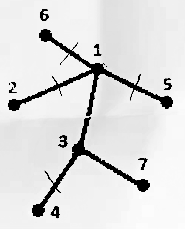
\includegraphics[width=0.13\linewidth]{./1}
\end{center}
\end{enumerate}

\section{Вариант 4 (август 2016, пересдача)}
\begin{enumerate}
\item Сформулируйте необходимое условие существования матрицы Адамара порядка $n$.
\item Чему в точности равно многоцветное число Рамсея $R_3(3, 13, 3)$?
\item Дайте определение дистанционного графа в $\mathbb{R}^n$.
\item Сколько существует различных деревьев на данных $10$ вершинах?
\item Чему равно число независимости $\alpha(KG_{10, 4})$, где $KG_{10, 4}$ --- кнезеровский граф?
\item Выпишите, какая с.о.п. будет построена жадным алгоритмом для набора множеств $\{1,3,6\}; \{1,4,7\}; \{2,4,6\}; \{3,5,6\},\{2,5,7\}$ и~в~каком порядке будут включены в с.о.п. соответствующие элементы.
\item Исправьте ошибку в формулировке теоремы Эрдеша-Ко-Радо, если она есть.

Пусть $F$ - любое семейство $k$-элементных подмножеств $n$-элементного множества. Если $2k \geqslant n$ и объединение никаких двух подмножеств из $F$ не есть всё $n$-элементное множество, то $|F| \leqslant C_{n-1}^{k-1}$.
\item Вычислите перманент следующей матрицы: 
$$\begin{pmatrix}
1 & 1 & 0 & 1 \\
0 & 1 & 1 & 1 \\
1 & 0 & 1 & 1
\end{pmatrix}
$$
\end{enumerate}


\section{Вариант 5 (сентябрь 2016, пересдача)}
\begin{enumerate}
\item Исправьте ошибки в формулировке теоремы, если они есть. 

Для плоского графа $G$ справедлива формула Эйлера: $|V(G)| - |F(G)| + |E(G)| = 2$, где $|V(G)|$ --- количество вершин $G$, $|F(G)|$ --- количество граней $G$, а $|E(G)|$ --- количество ребер $G$.
\item Нарисуйте дерево с вершинами $1, 2, \ldots 6$, которому соответствует код Прюфера $2 1 3 3$.
\item Чему равно число Рамсея $R(K_10, K_2)$?
\item Какая асимптотика у функции $f(n) = \ln(n!)$ при $n\rightarrow \infty$?
\item Чему равно хроматическое число $\chi(KG_{6,3})$, где $KG_{n,k}$ - кнезеровский граф?
\item Дайте определение матрицы Адамара порядка $n$.
\item Сформулируйте теорему Эрдеша о графах с большим обхватом и большим хроматическим числом.
\item Добавьте к совокупности $\{\{1, 3\}; \{4, 5\}; \{1, 2, 3\}; \{1, 4, 5, 6\}; \{2, 3 ,4\}; \{1, 2, 4, 5\}; \{2, 3\}\}$ такое множество, чтобы новая совокупность дробила множество $\{1, 2, 4\}$.
\end{enumerate}

\chapter{2017 год}

\section{Вариант 1 (июнь 2017)}
\begin{enumerate}
\item Сформулируйте теорему Холла.
\item Чему равно двудольное число Рамсея $b(1,7)$?
\item Дайте определение дистанционного графа в $\mathbb{R}^n$
\item Исправьте ошибку в формулировке теоремы Эрдеша-Ко-Радо, если она есть.

\textit{Пусть $F$ --- любое семейство $k$-элементных подмножеств $n$-элементного множества. Если $2k \leqslant n$ и любые два подмножества из $F$ пересекаются, то $|F| \leqslant C_n^k$.}
\item Приведите пример матрицы Адамара, первый столбец которой есть $(1, -1, -1, 1)^T$.
\item Приведите асимптотику функции $\ln n!$ при $n \rightarrow \infty$.
\item Какое максимальное количество вершин может быть в графе с хроматическим числом $\chi(G) = 5$ и числом независимости $\alpha(G) = 5$?
\item Является ли последовательность $1100010111$ последовательностью де Брейна? Если является, то напишите, чему равны ее порядок $n$ и мощность алфавита $k$, если нет, то обоснуйте, почему.
\end{enumerate}

\section{Вариант 2 (август 2017, пересдача)}
\begin{enumerate}
\item Исправьте ошибки в формулировке теоремы, если они есть.

\textit{Пусть $\displaystyle p = \frac{\ln n + c + o(1)}{n}$, тогда $P(G_{n,p}\,\, \text{связен}) \rightarrow e^{-c}$, при $n \rightarrow \infty$ (где $G_{n,p}$ --- случайный граф в модели Эрдеша-Реньи).}
\item Чему равно двудольное число Рамсея $b(1, 5)$?
\item Дайте определение кнезеровского графа $KG_{n, k}$.
\item Сформулируйте критерий эйлеровости графа (вида <<граф эйлеров тогда и только тогда, когда ...>>, а не теорему об эквивалентных условиях).
\item Приведите пример графа с числом независимости 5 и хроматическим числом 4.
\item С.о.п. какого размера наберет жадный алгоритм для гиперграфа со следующей матрицей инцидентностей (строки матрицы --- вершины, столбцы --- ребра):
$$
\begin{pmatrix}
1 & 1 & 0 & 0 & 0 & 1 \\
0 & 0 & 1 & 0 & 0 & 1 \\
1 & 0 & 0 & 1 & 0 & 0 \\
0 & 1 & 0 & 0 & 1 & 0
\end{pmatrix}?
$$
\item Найдите асимптотику функции $f(n) = C_{\sqrt{n}}^{\ln^2 n}$ при $n \rightarrow \infty$.
\item Какое минимальное количество множеств должно быть в совокупности, с помощью которой можно раздробить множество $\{2, 8, 13, 21, 35\}$?
\end{enumerate}

\section{Вариант 3 (сентябрь 2017, пересдача)}
\begin{enumerate}
\item Для каких из перечисленных кодов Прюфера существует дерево с вершинами $1, 2, \ldots, 8$ (нужное обвести): а)~$2, 6, 3, 3, 6, 1, 7$; b)~$4, 4, 4, 4, 4, 4$; c)~$2, 3, 9, 3, 4, 1$; d)~$1, 6, 4, 5, 3, 2$?
\item Чему равно число Рамсея $R(K_10, K_2)$?
\item Найдите минимальную с.о.п. для набора множеств
$$\{\{1,2,3,4\}; \{1,4,5\}; \{2,3,6\}; \{4,5,6\}; \{3,6\}; \{2,4,6\}; \{1,5\} \}.$$
\item Сформулируйте необходимое условие существования матрицы Адамара порядка $n$.
\item Приведите асимптотику $g(n)$ для функции $f(n) = \sqrt[n]{n!}$ при $n \rightarrow \infty$ (т.е. найдите <<явную>> функцию $g(n)$, для которой $f(n) \sim g(n)$ при $n \rightarrow \infty$).
\item Чему равно число независимости $\alpha(KG_{6,3})$, где $KG_{6,3}$ --- кнезеровский граф?
\item Сформулируйте теорему Эрдеша о графах с большим обхватом и большим хроматическим числом.
\item Дайте определение величине $\chi(\mathbb{R}^n)$.
\end{enumerate}

\chapter{Ответы}

В дебильнике требуется только указать ответ. Обратите внимание, что ответы, помеченные звездочкой~(\textbf{*}),  предоставлены <<сообществом>> и не были верифицированы непосредственно на экзамене. Если звездочки нет, значит, за данный ответ в \textit{реальной} работе был поставлен <<+>>. Сообщайте обо всех найденных ошибках/опечатках!

~

\textbf{Контакты}:

Telegram: @celidos

\url{https://github.com/celidos/TEX}

\url{https://vk.com/eddie\_mur}

\section{2015}
\subsubsection{Вариант 1}

\textbf{1*.}~Например, $\{\{1,2,3,4,5\}; \{1,2,6,7,8\}\}$.
\textbf{2*.}~$20^{18}$. Условие подходит к определению дерева, используем формулу Кэли.
\textbf{3*.}~Связный граф содержит в себе эйлеров путь тогда и только тогда, когда степень каждой его вершины четна.
\textbf{4*.}~$8$. Первая строка состоит из единиц. Все остальные строки ортогональны ей, значит, каждая содержит по $8/2 = 4$ единицы и по $4$ минус единицы. Значит, сумма элементов в любой строке, кроме первой, равна $0$.
\textbf{5.}~Например, <<Y>>-образный граф на 4 вершинах.
\textbf{6.}~
\textbf{7*.}~$\infty$.
\textbf{8*.}~$f(n) = 1{,}5^n$. Напомним, что запись $f(n) = o(g(n))$ означает, что $\displaystyle \lim_{n \to \infty}\frac{f(n)}{g(n)} = 0$. Но $\displaystyle \lim_{n \to \infty}\frac{1{,}5^n}{{2}^{n}} = \lim_{n \to \infty}\left(\frac{1{,}5}{2}\right)^n = 0 \Rightarrow 1{,}5^n = o(2^n)$. В~то же время $\displaystyle \lim_{n \to \infty}\frac{n^{2 \ln n}}{1{,}5^n} = \lim_{n \to \infty}\frac{1{,}5^{2 \ln n \cdot \log_{1{,}5} n}}{1{,}5^n} = 0 \Rightarrow n^{2 \ln n} = o(1{,}5^n)$, т.~к. $2 \ln n \cdot \log_{1{,}5} n$ растет медленнее, чем $n$.

\subsubsection{Вариант 2}

\textbf{1.}~
\textbf{2.}~
\textbf{3.}~
\textbf{4.}~
\textbf{5??.}~$59$.
\textbf{6.}~
\textbf{7.}~
\textbf{8.}~

\subsubsection{Вариант 3}

\textbf{1.}~$\chi(G) \geqslant \omega(G)$.
\textbf{2.}~Если в связном графе $n$ вершин и  степень любой вершины $\geqslant \frac{n}{2}$, то этот связный граф --- гамильтонов.
\textbf{3.}~Например, <<Y>>-образный граф на 4 вершинах.
\textbf{4.}~$6 \cdot 5 \cdot 4 \cdot 4 = 480$.
\textbf{5.}~$\displaystyle \frac{1}{3} \cdot \left(1-\frac{1}{3}\right)^{98} \left(1-\frac{1}{3}\right)^{98}$.
\textbf{6.}~$\infty$. Применяем формулу Стирлинга, откуда остаётся лишь $2\sqrt{n\pi}$, дальше очевидно.
\textbf{7.}~$9$. Больше 10 мы не получим, т.к. $|A| = 10$, при этом $10$ не достигается, т.~к. невозможно высечь пустое множество, для 9 все работает.
\textbf{8.}~2. Здесь можно применить правило <<0 лучше 1 лучше 2>>.
\subsubsection{Вариант 4}

\textbf{1.}~Например, $\{\{1,2,3\}; \{1,2,4\}; \{1,2,5\}\}$.
\textbf{2.}~$25^{23}$. Условие подходит к определению дерева, поэтому считаем по формуле Кэли.
\textbf{3.}~
\textbf{4.}~
\textbf{5.}~Например, <<Y>>-образный граф на 4 вершинах.
\textbf{6.}~
\textbf{7.}~$VC(\mathbb{N}, F) = \infty$.  
\textbf{8.}~
\subsubsection{Вариант 5}

\textbf{1.}~
\textbf{2.}~
\textbf{3.}~
\textbf{4.}~
\textbf{5.}~
\textbf{6.}~
\textbf{7.}~
\textbf{8.}~

\subsubsection{Вариант 6}

\textbf{1.}~2.
\textbf{2*.}~$n - e + f = 2$, где $n = |V|$, $e = |E|$, $f$ --- число граней.
\textbf{3.}~3. Заметим, что для простых циклов ответ зависит лишь от четности $n$: если $n$ четно, то $\chi(G) = 2$, иначе $\chi(G) = 3$.
\textbf{4.}~$R(n, n) \geqslant \displaystyle (1+o(1)) \frac{\sqrt{2}}{e}n2^{n/2}$ (теорема Спенсера).
\textbf{5.}~8. Можно выписать любую  подходящую матрицу, дальше по формуле разложения по строке.
\textbf{6.}~$17 = 4^2 + 2 - 1$.
\textbf{7.}~0.
\textbf{8.}~0.

\section{2016}
\subsubsection{Вариант 1}

\textbf{1.}~<<b>> и <<d>>.  В случае <<a>> последовательность слишком длинная, <<c>> --- не м.б. вершины с номером 9.
\textbf{2.}~Пусть у графа $G = (V, E)$ число вершин $|V| = n$ и $\alpha = \alpha(G)$. Тогда в этом графе \mbox{$\displaystyle |E| \geqslant n\left[\frac{n}{\alpha}\right] - \left[\frac{n}{\alpha}\right]\left[\frac{n}{\alpha} + 1\right]\cdot\frac{\alpha}{2}$}.
\textbf{3*.}~$8^4 = \sqrt{8^8}$.  Известно, что $A \cdot A^T = nE \Rightarrow \det(AA^T) = n^n$.
\textbf{4.}~$C_{16}^8 \geqslant \frac{2^{16}}{17}$.
\textbf{5.}~$R(3, 2, 4)=R(3, 4) = 9$.
\textbf{6.}~$m(n, k, t) = \max\{m \in \mathbb{N}\,\colon\,\exists\,k\text{-однородный гиперграф } H = (V, E), |V| = n, |E| = m, \forall A, B \in E \colon |A \cap B| \neq t \}$.
\textbf{7.}~$\left(\frac{1}{3}\right)^{C_k^2}$.
\textbf{8.}~

\subsubsection{Вариант 2}

\textbf{1.}~$R(C_3, K_4) = R(3, 4) = 9$.
\textbf{2.}~4 (все вершины). \textit{Прим.:} сначала алгоритм возьмет первую вершину, т.~к. в первой строке больше всего единиц.
\textbf{3.}~$\chi \geqslant 3$, $\chi \leqslant 7$.
\textbf{4.}~Cуществует такой набор точек $A$ в $\mathbb{R}^n$, что $|A|=n+2$, $A \subset \mathbb{R}^n$, и $\exists U, V\, \colon\,A = U \sqcup V$  и $\text{conv}(U) \cap \text{conv}(V) \neq \varnothing$.
\textbf{5.}~$\chi(\mathbb{R}^n) = \min\{k\,\colon\,\mathbb{R}^n=V_1\sqcup\ldots\sqcup V_k \text{ и } \forall i \,\, \forall u, v \in V_i \,\, \rho(u, v) \neq 1 \}$.
\textbf{6.}~8. Используйте формулу $n - e + f = 2$.
\textbf{7.}~
\textbf{8.}~$f(n, k, 1) = C_{n-1}^{k-1}$ при $k \leqslant \frac{n}{2}$, где $f(n, k, 1) = \max\{m \in \mathbb{N}\,\colon\,\exists\,k\text{-однородный гиперграф } H = (V, E), |V| = n, |E| = m, \forall A, B \in E \colon |A \cap B| \geqslant 1 \}$. \textit{Прим.:} лучше написать определение $f(n, k, t)$, иначе могут не засчитать.

\subsubsection{Вариант 3}

\textbf{1.}~$G = (V, E)$ --- эйлеров $\Leftrightarrow$ $G$ связен и $\forall v \in V\, \deg v \equiv 0 \,\,\,\,(\text{mod } 2)$. \textit{Прим.:} Связность, связность, связность!
\textbf{3.}~Гиперграф, в котором $\forall e, f \in E\,\,|e \cap f| \geqslant t$.
\textbf{4.}~$\{1, 4, 9\}$.
\textbf{5.}~$R(K_3, K_3) = 6$, $\alpha(K_{6, 9}) = 9$, $\chi(C_{11}) = 3$, поэтому $\alpha(K_{6, 9}) > R(K_3, K_3) > \chi(C_{11})$.
\textbf{6*.}~Пусть $A_1, \ldots, A_n$ --- события на $(\Omega, \mathscr{F}, \mathbf{P})$. Пусть $\forall i\,\, \mathbf{P}(A_i) \leqslant p < 1$ и $\forall i \,\,A_i$ не зависит от совокупности всех остальных событий, кроме не более $d$ штук, и числа $p$, $d$ не зависят от $i$. Тогда, если $ep(d+1)<1$, то $\displaystyle \mathbf{P}\left( \bigcap_{i=1}^{n} \overline{A_i}\right) > 0$.
\textbf{7.}~$2^4 = 16$.
\textbf{8.}~$1 3 1 1 3$.

\subsubsection{Вариант 4}

\textbf{1.}~
\textbf{2.}~
\textbf{3.}~
\textbf{4.}~
\textbf{5.}~
\textbf{6.}~
\textbf{7.}~
\textbf{8.}~

\subsubsection{Вариант 5}

\textbf{1.}~
\textbf{2.}~
\textbf{3.}~
\textbf{4.}~
\textbf{5.}~
\textbf{6.}~
\textbf{7.}~
\textbf{8.}~

\section{2017}
\subsubsection{Вариант 1}

\textbf{1.}~Пусть $S_1, \ldots, S_m$ --- конечные множества. $\forall i \in \{1, \ldots, m\}$ можно выбрать $x_i \in S_i$ так, чтобы $\forall i, j\,\,\,x_i \neq x_j$ при $(i \neq j)$, если $\forall k \in \{1, \ldots, m\}$ объединение любых $k$ множеств из $S_1, \ldots, S_m$ содержит $\geqslant k$ элементов.
\textbf{2.}~7.
\textbf{3.}~
\textbf{4.}~$|F| \leqslant C_{n-1}^{k-1}$.
\textbf{5.}~$\begin{pmatrix}
1 & 1 & 1 & 1 \\
-1 & 1 & -1 & 1 \\
-1 & -1 & 1 & 1 \\
1 & -1 & -1 & 1
\end{pmatrix} = \begin{pmatrix}
1 & 1 \\
-1 & 1
\end{pmatrix} \otimes \begin{pmatrix}
1 & 1 \\
-1 & 1
\end{pmatrix}$. См. получение матриц Адамара кронекеровским произведением.
\textbf{6.}~$\ln n! \sim n \ln n$.
\textbf{7.}~$|V| \leqslant 25$. Используйте $\chi(G) \geqslant \frac{|V|}{\alpha(G)}$. 
\textbf{8.}~Является, $k = 2$, $n = 3$.

\subsubsection{Вариант 2}

\textbf{1.}~$P(G_{n,p} \,\,\text{связен}) \rightarrow e^{-e^{-c}}$
\textbf{2.}~5.
\textbf{3.}~Кнезеровским графом $KG_{n, k} = (V, E)$ называется граф такой, что $V$ --- все $k$-элементные подмножества $\{1, \ldots, n\}$, а $E = \{(A, B)\,\colon\,\,A \cap B = \varnothing\}$.
\textbf{4.}~
\textbf{5.}~Подойдет  <<$5K_4$>> или <<$K_4$ и четыре изолированные вершины>>.
\textbf{6.}~4.
\textbf{7.}~
\textbf{8.}~$2^5 = 32$.

\subsubsection{Вариант 3}

\textbf{1.}~<<b>> и <<d>>.
\textbf{2.}~$10$.
\textbf{3.}~$\{1, 6\}$.
\textbf{4.}~Если при заданном $n$ существует матрица Адамара порядка $n$, то $n=1$ или $n=2$ или $n$ делится на $4$ при $n > 3$. \textit{Прим.:} не путать необходимое (<<если существует, то $n \ldots$>>) и достаточное условие (гипотеза Адамара -- <<если $n \ldots$, то существует>>)!
\textbf{5.}~$g(n) = \frac{n}{e}$.
\textbf{6.}~$\alpha(KG_{6,3}) = 10 = f(6, 3, 1) = C_{6-1}^{3-1}$.
\textbf{7.}~$\forall k, l$ существует граф, у которого обхват $\geqslant k$, а хроматическое число $\geqslant l$.
\textbf{8.}~$\chi(\mathbb{R}^n) = \min\{k\,\colon\,\mathbb{R}^n=V_1\sqcup\ldots\sqcup V_k \text{ и } \forall i \,\, \forall u, v \in V_i \,\, \rho(u, v) \neq 1 \}$.

\end{document}